
The small signal gain ($g_m$) and the cut-off frequency ($F_t$) of the transistor are both important in digital and analog circuits. 
A higher small signal gain means that the analog circuitry requires less transistors for the same amplification factor, reducing the circuits size and parasitics. 
The increase of the small signal gain also increases the current output strength of digital gates, helping in the charge and discharge of capacitive loads, such as gates or PN junctions. 
The other parameter, the cut-off frequency of the transistor, is a measurement of how fast a single transistor can switch.
Improving the cut-off frequency of the transistor opens up the design area for analog and digital circuitry as it represents the upper limit at which a circuit can run in a parasitic-less environment. 
The saturation region small signal gain is the measurement of how much the drain current ($I_D$) changes in relation to the gate-to-source voltage ($V_{GS}$) in a specific condition of the drain-to-source voltage ($v_{DS}$).

\begin{equation}
\label{eq:gm}
g_m = \left.\frac{\delta I_D}{\delta V_{GS}}\right|_{v_{DS}} = \mu_x C_{ox}\frac{W}{L}(V_{GS}-V_T)(1+\lambda v_{DS})
\end{equation}

In \ref{eq:gm}, $\mu_x$ is the mobility of the charges, $C_{ox}$ is the oxide capacitance per unit area, $W$ and $L$ are the size of the gate, $V_T$ is the threshold voltage and $\lambda$ is the channel-length modulation parameter. 
%In  conventionnal silicon photonics process, the $W$ value is the height of the waveguide, hence the designer only has access on controlling the bias point via  $V_{GS}$ via an external application, and the length $L$ and the oxide capacitance $C_{ox}$ up to their respective manufacturing limit.
The length of the transistor is controllable by the distance between two tubs of the same type of doping (Fig.\ref{fig:Core}.D, in red) and the length of the gate while the width is fixed by the waveguide layer height (see the $W$ and $L$ on Fig.\ref{fig:Core}.E).
%As the physical limit of the gate length is the minimal width of a silicon waveguide, the limiting factor is often the minimal distance between two tubs of similar doping without causing a unwanted connection between the source and the drain.
Depending on the foundry, the minimal $L$ distance can vary and is subject to mask alignment precision but should be used for maximum $g_m$ value. 
As for maximizing $C_{ox}$, reducing the gap between the channel and the gate to the foundry's limit is the way to go, as one cannot easily change the material used between silicon waveguides. 
%it is not only found in \ref{eq:gm} but also in the formula of $V_T$, which influences the bias point and $g_m$.

%\begin{equation}
%\label{eq:Vt}
%V_T = V_{fb} + 2\phi_F + \frac{\sqrt{2\varepsilon_{Si} qN(2\phi_F)}}{C_{ox}}
%\end{equation}

%In (\ref{eq:Vt}), $V_{fb}$ is the flat band voltage,  $\phi_F$ is fermi potential of the doped channel, $\varepsilon_{Si}$ the permitivity of silicon, $q$ the elemental charge and $N$ the doping of the channel.
%It is better to increase the $C_{ox}$ value as much as possible, as it has the double effect of reducing the $V_T$ in (\ref{eq:Vt}) and increasing the $gm$ from (\ref{eq:gm}).

The second metric, the cut-off frequency $F_T$, is defined by the small-signal gain over its gate-source ($C_{GS}$) and gate-drain capacitance ($C_{GD}$).

\begin{equation}
\label{eq:Ft}
F_t = \frac{g_m}{2\pi(C_{GS}+C_{GD})} = \frac{\mu_x(V_{GS}-V_t)}{2\pi (\frac{2}{3}L^2+2L_{ov}L)},
\end{equation}

where $L_{ov}$ is the overlap length between the gate and the source or drain area.
Together with the diminution of the $L$ value, one could theoretically increase the maximum frequency of operation up to 25 GHz and the $g_m$ up to 4 $\mu$A/V as shown in Fig.\ref{fig:ft} and Fig.\ref{fig:gm}.
Both $g_m$ and $F_t$ are subject to carrier velocity saturation at shorter $L$ values. 

\begin{figure}[h]
    \begin{minipage}{0.24\textwidth}
        \centering
        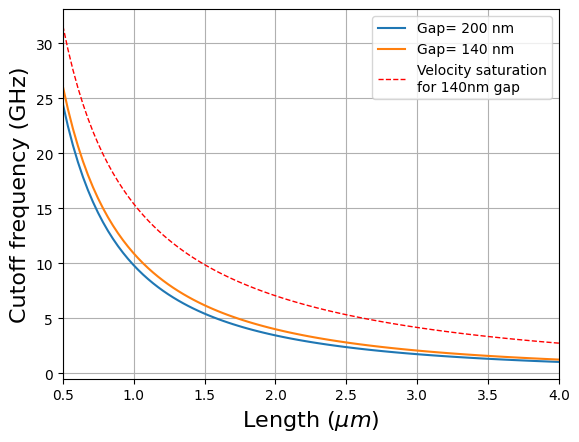
\includegraphics[width=\linewidth]{ft1.png}
        \caption{$F_t$ of a NMOS at $V_{gs}$ = 5V}
        \label{fig:ft}
        
    \end{minipage}%
    \hspace{0.1pt}
    \begin{minipage}{0.24
        \textwidth}
        \centering
        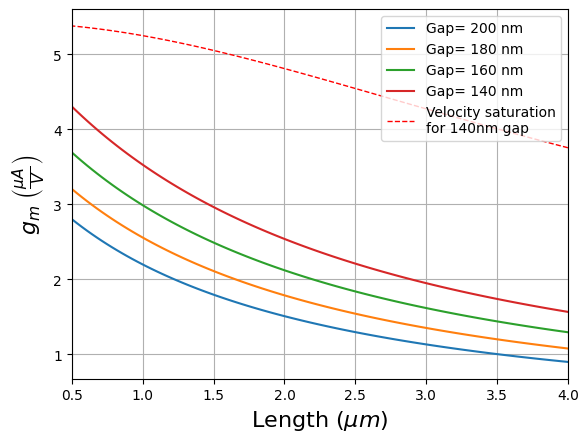
\includegraphics[width=\linewidth]{gm.png}
        \caption{$g_m$ of a NMOS at $V_{gs}$ = 5V}
        \label{fig:gm}
    \end{minipage}
\end{figure}





